\chapter{Architetture}
\color{red}
Nel campo dello sviluppo web, le tecniche di rendering svolgono un ruolo cruciale nel fornire esperienze utente coinvolgenti. Due approcci di rendering popolari sono il rendering lato client (CSR) e il rendering lato server (SSR).
Entrambi i metodi presentano vantaggi e considerazioni specifici, pertanto è importante che gli sviluppatori comprendano le differenze tra loro. In questo articolo esploreremo CSR e il rendering SSR, evidenziando le loro distinzioni e fornendo esempi rilevanti per chiarirne i casi d'uso.

\section{Server Side Rendering (SSR)}
\section{Client Side Rendering (CSR)}

\begin{figure}[H]
    \centering
    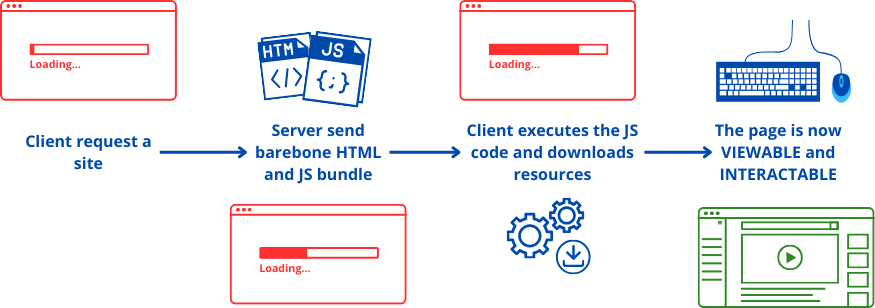
\includegraphics[width=0.7\textwidth]{architectures/CSR.png}
    \caption{Processo di rendering lato client (CSR)}
    \label{fig:CSR}
\end{figure}

Il CSR, o rendering lato client, è una tecnica in cui il processo di rendering avviene appunto sul client, in genere nel browser Web dell'utente.\\
In sintesi, il server invia un documento HTML minimo insieme ai file JavaScript al client. Il browser quindi esegue il
codice JavaScript, il quale è responsabile del recupero dei dati dalle eventuali API, della generazione e della
manipolazione del Document Object Model (DOM) per aggiornare l'interfaccia utente. \\
Nella figura \ref{fig:CSR} è mostrato il processo di rendering lato client.

\color{red}
\paragraph{Esempio di CSR:}
Consideriamo il feed di un social media che deve mostrare un elenco di post. Con CSR, l'HTML e il JavaScript iniziali
vengono inviati al client. Il codice JavaScript, eseguito sul client, recupera quindi i dati del post da un'API e li
visualizza dinamicamente nel browser dell'utente. Mentre l'utente scorre, altri post possono essere recuperati in modo
asincrono, consentendo una paginazione fluida senza dover ricaricare l'intera pagina.
\color{black}
\section{Architetture ibride}
\section{Confronto tra le architetture}
Scelta dell'approccio giusto
La scelta tra CSR e SSR dipende dai requisiti specifici del tuo progetto. Ecco alcune considerazioni chiave:
Complessità dell'applicazione: CSR è adatta per applicazioni dinamiche e altamente interattive, come applicazioni a pagina singola (SPA) o strumenti di collaborazione in tempo reale. SSR, d'altro canto, è adatta per siti Web o applicazioni incentrati sui contenuti che richiedono eccellenti prestazioni SEO.
Tempo per il primo rendering: se fornire un rapido caricamento iniziale della pagina è una priorità, SSR può essere vantaggioso. Tuttavia, se le interazioni successive e la reattività sono cruciali, CSR potrebbe essere la scelta migliore.
Sviluppo e manutenzione: CSR può essere più complesso da implementare e mantenere a causa della separazione della logica client e server. SSR semplifica lo sviluppo poiché richiede meno dipendenze JavaScript e consente un debug e un test più semplici.
Client-Side Rendering (CSR) e Server-Side Rendering (SSR) sono due importanti tecniche di rendering nello sviluppo web, ciascuna con i suoi vantaggi unici. CSR eccelle in interattività e prestazioni, mentre SSR offre vantaggi in SEO e prestazioni di caricamento iniziale.
Comprendendo le differenze e considerando i requisiti del tuo progetto, puoi prendere una decisione informata su quale approccio di rendering si adatta meglio alle tue esigenze.
Ricorda che esistono anche approcci ibridi, come Static Site Generation (SSG) e Incremental Static Regeneration (ISR), e possono fornire opzioni aggiuntive da esplorare per strategie di rendering ottimali in scenari specifici.


\color{black}